%%%%%%%%%%%%%%%%%%%%%%%%%%%%%%%%%%%%%%%%%
% Thesis 
% LaTeX Template
% Version 1.3 (21/12/12)
%
% This template has been downloaded from:
% http://www.latextemplates.com
%
% Original authors:
% Steven Gunn 
% http://users.ecs.soton.ac.uk/srg/softwaretools/document/templates/
% and
% Sunil Patel
% http://www.sunilpatel.co.uk/thesis-template/
%
% License:
% CC BY-NC-SA 3.0 (http://creativecommons.org/licenses/by-nc-sa/3.0/)
%
% Note:
% Make sure to edit document variables in the Thesis.cls file
%
%%%%%%%%%%%%%%%%%%%%%%%%%%%%%%%%%%%%%%%%%

%----------------------------------------------------------------------------------------
%	PACKAGES AND OTHER DOCUMENT CONFIGURATIONS
%----------------------------------------------------------------------------------------

\documentclass[11pt, a4paper, oneside]{Thesis} % Paper size, default font size and one-sided paper

\graphicspath{{./Pictures/}} % Specifies the directory where pictures are stored

\usepackage[comma, sort&compress]{natbib} % Use the natbib reference package - read up on this to edit the reference style; if you want text (e.g. Smith et al., 2012) for the in-text references (instead of numbers), remove 'numbers'
\usepackage[utf8]{inputenc}
\usepackage{float}
\usepackage{fancyvrb}
\usepackage[linesnumbered,ruled]{algorithm2e}
\usepackage{amsmath}
\usepackage{lingmacros}
\usepackage{rotating}
\hypersetup{urlcolor=black, colorlinks=true} % Colors hyperlinks in blue - change to black if annoying
\title{\ttitle} % Defines the thesis title - don't touch this

\begin{document}

\frontmatter % Use roman page numbering style (i, ii, iii, iv...) for the pre-content pages

\setstretch{1.3} % Line spacing of 1.3

% Define the page headers using the FancyHdr package and set up for one-sided printing
\fancyhead{} % Clears all page headers and footers
\rhead{\thepage} % Sets the right side header to show the page number
\lhead{} % Clears the left side page header

\pagestyle{fancy} % Finally, use the "fancy" page style to implement the FancyHdr headers

\newcommand{\HRule}{\rule{\linewidth}{0.5mm}} % New command to make the lines in the title page

% PDF meta-data
\hypersetup{pdftitle={\ttitle}}
\hypersetup{pdfsubject=\subjectname}
\hypersetup{pdfauthor=\authornames}
\hypersetup{pdfkeywords=\keywordnames}

%----------------------------------------------------------------------------------------
%	TITLE PAGE
%----------------------------------------------------------------------------------------

\begin{titlepage}
\begin{center}

\textsc{\LARGE \univname}\\[0.1cm]
\textsc{Faculteit der Natuurwetenschappen, Wiskunde en Informatica} \\[1cm] % University name
\textsc{\Large MSc Thesis}\\[0.5cm] % Thesis type

\HRule \\[0.4cm] % Horizontal line
{\huge \bfseries \ttitle}\\[0cm] % Thesis title
\HRule \\[1.5cm] % Horizontal line

\begin{minipage}{0.4\textwidth}
\begin{flushleft} \large
\emph{Author:}\\
\authornames % Author name - remove the \href bracket to remove the link
\end{flushleft}
\end{minipage}
\begin{minipage}{0.4\textwidth}
\begin{flushright} \large
\emph{Supervisor:} \\
\supname % Supervisor name - remove the \href bracket to remove the link  
\end{flushright}
\end{minipage}\\[3cm]
 
\large \textit{A thesis submitted in fulfillment of the requirements\\ for the degree of \degreename}\\[0.3cm] % University requirement text
\textit{in the}\\[0.4cm]
\deptname\\[2cm] % Research group name and department name

{\large \today}\\[2cm] % Date

\includegraphics[height=3cm]{uva-logo} % University/department logo - uncomment to place it

\vfill
\end{center}

\end{titlepage}

%----------------------------------------------------------------------------------------
%	DECLARATION PAGE
%	Your institution may give you a different text to place here
%----------------------------------------------------------------------------------------

%\Declaration{

%\addtocontents{toc}{\vspace{1em}} % Add a gap in the Contents, for aesthetics

%I, \authornames, declare that this thesis titled, '\ttitle' and the work presented in it are my own. I confirm that:

%\begin{itemize} 
%\item[\tiny{$\blacksquare$}] This work was done wholly or mainly while in candidature for a research degree at this University.
%\item[\tiny{$\blacksquare$}] Where any part of this thesis has previously been submitted for a degree or any other qualification at this University or any other institution, this has been clearly stated.
%\item[\tiny{$\blacksquare$}] Where I have consulted the published work of others, this is always clearly attributed.
%\item[\tiny{$\blacksquare$}] Where I have quoted from the work of others, the source is always given. With the exception of such quotations, this thesis is entirely my own work.
%\item[\tiny{$\blacksquare$}] I have acknowledged all main sources of help.
%\item[\tiny{$\blacksquare$}] Where the thesis is based on work done by myself jointly with others, I have made clear exactly what was done by others and what I have contributed myself.\\
%\end{itemize}
 
%Signed:\\
%\rule[1em]{25em}{0.5pt} % This prints a line for the signature
 
%Date:\\
%\rule[1em]{25em}{0.5pt} % This prints a line to write the date
%}

%\clearpage % Start a new page

%----------------------------------------------------------------------------------------
%	QUOTATION PAGE
%----------------------------------------------------------------------------------------

\pagestyle{empty} % No headers or footers for the following pages

\null\vfill % Add some space to move the quote down the page a bit

\textit{``Thanks to my solid academic training, today I can write hundreds of words on virtually any topic without possessing a shred of information, which is how I got a good job in journalism."}

\begin{flushright}
Dave Barry
\end{flushright}

\vfill\vfill\vfill\vfill\vfill\vfill\null % Add some space at the bottom to position the quote just right

\clearpage % Start a new page

%----------------------------------------------------------------------------------------
%	ABSTRACT PAGE
%----------------------------------------------------------------------------------------

\addtotoc{Abstract} % Add the "Abstract" page entry to the Contents

\abstract{\addtocontents{toc}{\vspace{1em}} % Add a gap in the Contents, for aesthetics

%From the project outline
A basic fact about human-human dialogue is that there is often more than one way of talking about any domain. For example, instead of saying \textit{``Turn right after 200 meters"}, a route giver may say \textit{``Turn right at Barclays"} given that \textit{``Barklays"} is an enstabilished referring expression. Human speakers efficiently align terminology and associated ontology in talking about any specific domain (in this example we can say that ontologically there is only one entity -- a location -- but there are different linguistic terms we can use to refer to it). In contrast, current dialogue systems typically have a static ontology and a static vocabulary, which is used in both generation and interpretation, requiring users to formulate their utterances using the terminology known by the system. The goal of this project is to work towards a system that adapts its own linguistic resources (including possible ontology, vocabulary and grammar) to the interlocutor. The system should be able to learn new concepts by assigning  new meanings to known words, as well as new words to talk about concepts known by the system in the domain.
}

\clearpage % Start a new page

%----------------------------------------------------------------------------------------
%	ACKNOWLEDGEMENTS
%----------------------------------------------------------------------------------------

\setstretch{1.3} % Reset the line-spacing to 1.3 for body text (if it has changed)

\acknowledgements{\addtocontents{toc}{\vspace{1em}} % Add a gap in the Contents, for aesthetics

The acknowledgements and the people to thank go here\ldots

% Other people to acknowledge
% - The guy who created this template: http://www.latextemplates.com/template/masters-doctoral-thesis
}
\clearpage % Start a new page

%----------------------------------------------------------------------------------------
%	LIST OF CONTENTS/FIGURES/TABLES PAGES
%----------------------------------------------------------------------------------------

\pagestyle{fancy} % The page style headers have been "empty" all this time, now use the "fancy" headers as defined before to bring them back

\lhead{\emph{Contents}} % Set the left side page header to "Contents"
\tableofcontents % Write out the Table of Contents

\lhead{\emph{List of Figures}} % Set the left side page header to "List of Figures"
\listoffigures % Write out the List of Figures

%\lhead{\emph{List of Tables}} % Set the left side page header to "List of Tables"
%\listoftables % Write out the List of Tables

%----------------------------------------------------------------------------------------
%	ABBREVIATIONS
%----------------------------------------------------------------------------------------

\clearpage % Start a new page

\setstretch{1.5} % Set the line spacing to 1.5, this makes the following tables easier to read

\lhead{\emph{Abbreviations}} % Set the left side page header to "Abbreviations"
\listofsymbols{ll} % Include a list of Abbreviations (a table of two columns)
{
\textbf{AI} & \textbf{A}rtificial \textbf{I}ntelligence \\
\textbf{ASR} & \textbf{A}utomatic \textbf{S}peech \textbf{R}ecognition \\
\textbf{CA} & \textbf{C}onversational \textbf{A}gent \\
\textbf{DM} & \textbf{D}ialogue \textbf{M}anager \\
\textbf{DP} & \textbf{D}ialogue \textbf{P}artner \\
\textbf{ISU} & \textbf{I}nformation \textbf{S}tate \textbf{U}pdate \\
\textbf{LU} & \textbf{L}anguage \textbf{U}nit \\
\textbf{ML} & \textbf{M}achine \textbf{L}earning \\
\textbf{MT} & \textbf{M}achine \textbf{T}ranslation \\
\textbf{NLP} & \textbf{N}atural \textbf{L}anguage \textbf{P}rocessing \\
\textbf{SLU} & \textbf{S}poken \textbf{L}anguage \textbf{U}nderstanding \\
\textbf{TDM} & \textbf{T}RINDIKIT \textbf{D}ialogue \textbf{M}anager \\
\textbf{TTS} & \textbf{T}ext \textbf{T}o \textbf{S}peech \\
%\textbf{Acronym} & \textbf{W}hat (it) \textbf{S}tands \textbf{F}or \\
}

%----------------------------------------------------------------------------------------
%	SYMBOLS
%----------------------------------------------------------------------------------------

\clearpage % Start a new page

\lhead{\emph{Symbols}} % Set the left side page header to "Symbols"

\listofnomenclature{lll} % Include a list of Symbols (a three column table)
{
$c$ & chunk of text \\
$m$ & meaning \\
$s$ & sentence \\
% Symbol & Name & Unit \\

& & \\ % Gap to separate the Roman symbols from the Greek

$\sigma$ & chunk similarity \\
$\tau$ & word similarity \\
% Symbol & Name & Unit \\
}

%----------------------------------------------------------------------------------------
%	DEDICATION
%----------------------------------------------------------------------------------------

%\setstretch{1.3} % Return the line spacing back to 1.3

%\pagestyle{empty} % Page style needs to be empty for this page

%\dedicatory{For/Dedicated to/To my\ldots} % Dedication text

%\addtocontents{toc}{\vspace{2em}} % Add a gap in the Contents, for aesthetics

%----------------------------------------------------------------------------------------
%	THESIS CONTENT - CHAPTERS
%----------------------------------------------------------------------------------------

\mainmatter % Begin numeric (1,2,3...) page numbering

\pagestyle{fancy} % Return the page headers back to the "fancy" style

% Include the chapters of the thesis as separate files from the Chapters folder
% Uncomment the lines as you write the chapters

% Chapter Template

\chapter{Introduction} % Main chapter title

\label{ch:Introduction} % Change X to a consecutive number; for referencing this chapter elsewhere, use \ref{ChapterX}

\lhead{\emph{Introduction}} % Change X to a consecutive number; this is for the header on each page - perhaps a shortened title

%----------------------------------------------------------------------------------------
%	INTRO TEXT
%----------------------------------------------------------------------------------------


The \textbf{user interface}, or human-computer interface, is the component of a computer system that provides a space of interaction between the human user and the resources offered by the machine; such a space defines a bridge language which human intentions can be translated into, to be converted into computational procedures for the machine; vice versa, the result of the computation is then presented to the user in the same language, which he or she is assumed to understand.

% cite Tanenbaum
In the early days of computing, the so-called \textbf{batch interfaces} were non-interactive: the user/programmer was supposed to feed the machine with a software, punched on cards using the \textit{machine's assembly language} directly, and retrieve the result of the computation printed on paper. The third and fourth generations of computing brought \textbf{text-based} interfaces for operating systems (UNIX, DOS, CP/M), that were later taken over by \textbf{Graphical User Interfaces} (GUI), moving the human-machine interaction on a new, visual language made of windows, icons and buttons. Recently, touch screen and camera devices allowed for the implementation of even more natural means of interaction based on \textbf{gestures} and physical actions.

From this brief spot on computing history, and in a way from common sense, we can draw the rather trivial, yet crucial, conclusion that the trend in user interfaces development is to \textbf{close the gap} between humans and machines by moving the needle of the interface languages from a machine-centered space towards the human language itself. To this respect, the studies on Natural Language Processing (NLP) assume a dramatically central role, as dramatically central is natural language in the interaction of humans with each other.

For this reason, the focus of this thesis work is the area of \textbf{dialogue systems}.

%----------------------------------------------------------------------------------------
%	DIALOGUE SYSTEM
%----------------------------------------------------------------------------------------

\section{General Architecture of a Dialogue System}
A dialogue system, or conversational agent (CA), is a computer software that allows humans and machines to interact through an intermediate language which is as close as possible to the \textbf{human language}, and through conversational episodes that implement as close as possible the human dialogue modalities.

The \textbf{basic architecture} of a dialogue system is shown in Figure \ref{ds_arch}. The figure represents the flow of information during the interaction between the system and a human user.

\begin{figure}
	\centering
	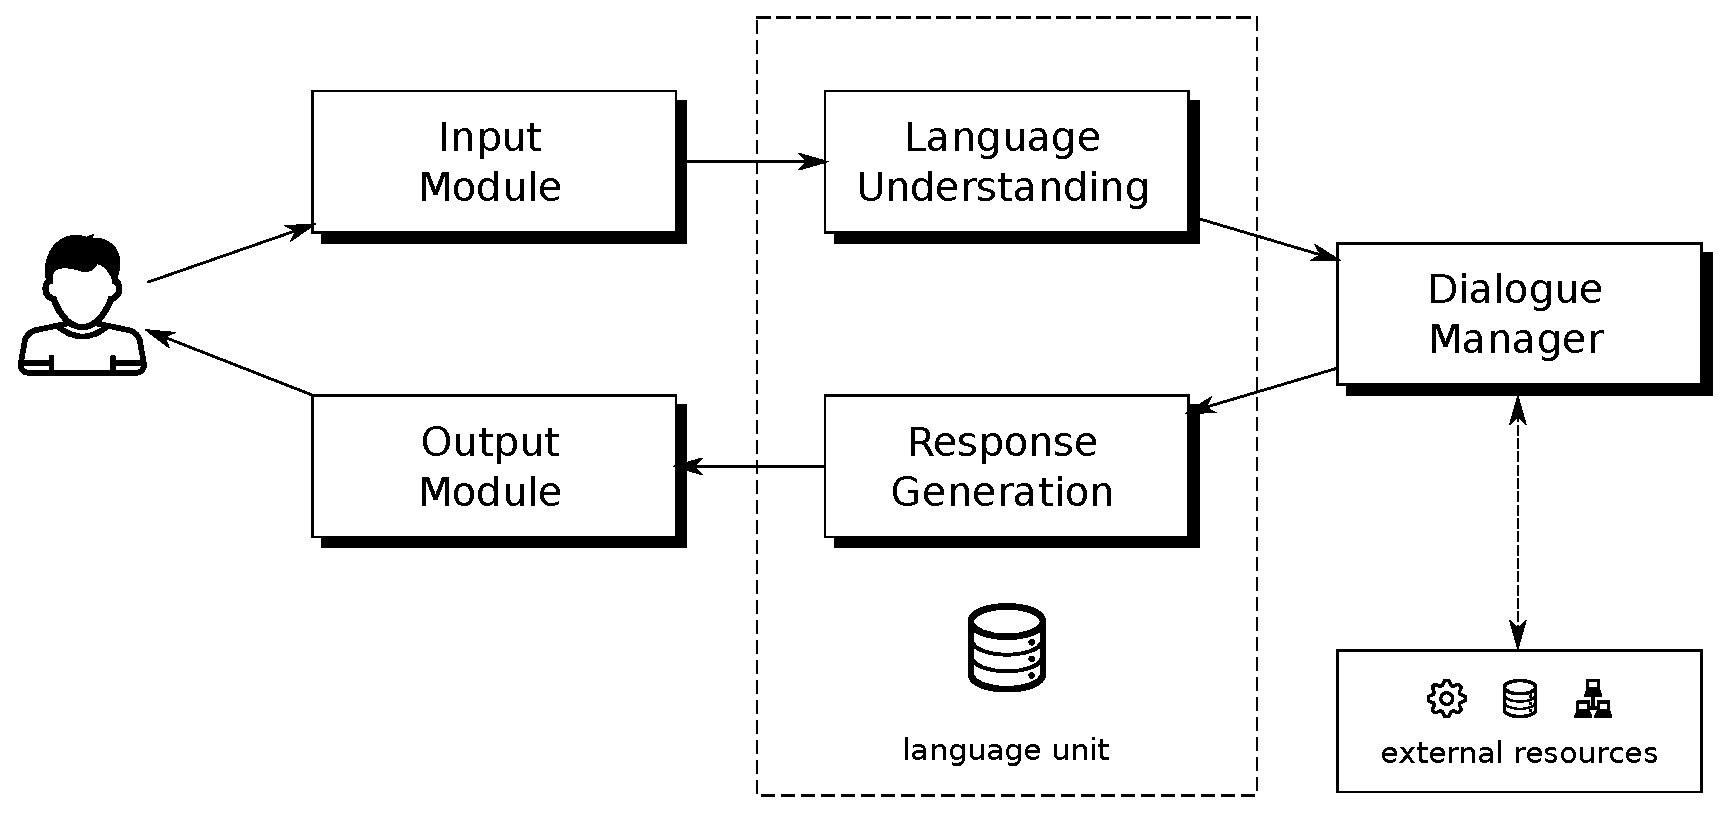
\includegraphics[width=15cm]{Pictures/ds_arch.pdf}
	\caption{The basic architecture of a dialogue system}
	\label{ds_arch}
\end{figure}
 
 \begin{enumerate}
	\item The user produces a dialogue act to be entered in the system, that receives it through its \textbf{input module}. As an example, the user may start a conversation by asking \textit{``What's your name?"}. Note that, although we will only address text-based interaction, spoken dialogue systems exist, where the input module is an Automatic Speech Recognition software.
	\item The \textbf{language understanding} module receives the user utterance, and interprets it into a logical form that the system can work with. In the previous example, the language understanding module would receive the string \texttt{"What's your name"} as input, and may output something like \texttt{"ask(?X.my\_name(X))"}.
	\item The result of the interpretation is given to the \textbf{dialogue manager} (DM). This component is the core of the system, as it has to model and keep track of the dialogue context and, within this context, integrate the user moves and plan the system answers. The dialogue manager can also access external resources in order to satisfy the user requests. In the example, the DM receives the interpreted user move \texttt{"ask(?X.my\_name(X))"}; its will then process this information, which broadly means:
	\begin{enumerate}
		\item Update the context, to include the pending user request.
		\item Find an answer for the user request
		\item Output the answer in the form of a system move (in the example, \\ \texttt{"answer(my\_name(`HAL9000'))"})
	\end{enumerate}
	\item The system move is received by the \textbf{response generation} module, whose purpose is to express that move with a natural language sentence, In the example, a proper output would be the string \texttt{"My name is HAL9000"}.
	\item Finally, the response string is received by the \textbf{output module}, which presents it to the user. This module can simply print the sentence on the screen, but it can also implement Text-To-Speech technology to allow spoken interaction with the user.
\end{enumerate}

As we will see in the next chapters, our work will be focused on the language understanding and response generation modules, that together form what we call the \textbf{Language Unit}. Our goal is to implement advanced language understanding and learning capabilities for this part of the system\footnote{This also includes minor modifications to the dialogue manager, as it will be explained in Chapter \ref{ch:interaction}}. 
 
Research on dialogue systems has been carried on since the \textbf{early days} of Artificial Intelligence. A milestone in the early work on this field is ELIZA \citep{Weizenbaum:1966:ECP:365153.365168}, which provides the user with a basic human-like interaction based on pattern matching; Figure \ref{ch:rw:ds:ELIZA} shows an instance of these patterns.

Another example is the SHRDLU system \citep{winograd1971procedure}, which interfaces the user with a simple spatial domain by listening to the user's utterances (e.g.\ ``Would you please put the green pyramid in the box?"), and performing actions accordingly in the domain, resolving, if necessary, ambiguous or implicit references to the entities in it.

\begin{figure}
\begin{Verbatim}[frame=single]
["dream", 3, [
 ["*", [
     "What does that dream suggest to you ?",
     "Do you dream often ?",
     "What persons appear in your dreams ?",
     "Do you believe that dreams have something to do
      with your problem ?"
  ]]
]]
\end{Verbatim}
\caption{One of the patterns included in ELIZA's DOCTOR script. It simply tells the system that the user input can be answered with any of the given sentences, whenever it contains the word ``dream".}
\label{ch:rw:ds:ELIZA}
\end{figure}

According to \cite{Jokinen2009}, modern dialogue systems can be divided in \textbf{two main types}: task-oriented and nontask-oriented. Intuitively, systems in the first category are meant to deal with a specific task such as making a hotel booking, or booking a plane ticket; an example in this category is the MIT Mercury system, a vocal interface to a flight database \citep{Seneff:2000:DMM:1605285.1605288}. On the other hand, nontask-oriented systems are meant to engage in conversations without a specific purpose to fulfill, but the one of delivering a realistic simulation; ELIZA itself is an example of nontask-oriented dialogue system.

Task-oriented systems can be very simple, as simple and well-formalized the task is;  many applications, such as travel service or call routing, can be successfully solved by \textbf{slot-based} systems: each step of the conversation requires some pieces of information, modeled as slots, to be filled in by the user (departure city, arrival city, date, and so on); given the slots to be filled, the dialogue task can be solved with a formal grammar of interaction. As the complexity increases, more phenomena of human interaction have to be modeled, such as turn-taking, multimodality or grounding
%\ignore{CITE RAQUEL'S CHAPTER}
, as well as semantic structures such as quantification and negation; slot-based systems are not sufficient to model these scenarios \citep{Gabsdil03clarificationin}, that require more advanced frameworks such a the Information State Update (ISU) one, which will be tackled in \ref{ch:rw:ds:isu}.

%----------------------------------------------------------------------------------------
%	LEARNING TO TALK
%----------------------------------------------------------------------------------------

\section{Learning to talk}

One of the constituent features of humans' ability to speak is that such an ability doesn't come fully developed in children, but rather \textbf{grows} with time, influenced by the interaction of the subject with the outer world.
%~ One of the constituent features of humans' ability to speak is that such an ability is \textbf{not innate}, but is rather learned through interactions.

Ever since the power of computers grew enough to allow for intensive statistical analysis of significant amounts of data, \textbf{Machine Learning} approaches to Artificial Intelligence tasks got more and more prominent in the scene, often outperforming static methods (i.e. where the solution procedure for a task is explicitly coded by the programmer).
% Citation needed...
One of the clearest examples is the field of NLP itself, where the most important tasks, like parsing or machine translation, are dominated by Machine Learning methods based on corpora,
% Citation needed
meaning that, for instance, a Machine Translation system will first be trained on a corpus of aligned sentences. Statistical structures will be extracted from this corpus, like the most likely word-by-word alignment, and later be used to process new examples.

However, the task of learning through dialogue interactions comes with some \textbf{peculiar} challenges. First of all, humans learning to talk do not go through two separate phases of learning and processing, but rather improve their abilities episode by episode; as \cite{2095408} point out, this \textbf{incremental learning} structure is nowadays not implemented in state-of-the-art systems. Also, the nature of this incrementing learning is \textbf{not linear}, as the new information was stacked little by little on the existing one: new words and phrases can be described with concepts and linguistic structures that are already present in the learner's mind. Lastly, if we keep considering the way humans learn to talk, we realize that, as from a certain point, the language ceases to be a mere subject of learning, and \textbf{becomes the means} by which it is itself learned: the same linguistic structures that are used to express concepts and categories of the learner's experience, can also be used to describe themselves, as they become part of the same experience; we can observe a clear example of this process in any primary-school-level English class, where the teacher explains, by using English sentences, how English sentences are structured.

We can identify some \textbf{ideal features} we would like to have implemented into an automatic language learner:
\begin{itemize}
	\item Learning to produce or understand new surface forms, or \textbf{realizations}, for a given meaning -- eg. the sentence ``Bill eats an apple" for the action of Bill eating an apple.
	\item Learning to produce new \textbf{meanings} from the existing ones and their respective realizations -- eg. the concept of motor home, sharing the features of a house and a car.
	\item Learning a \textbf{``grammar" of conversation}, to place the correct utterance at each step of a conversational episode. -- eg. an appropriate answer to the utterance ``My name is Bill" can be ``Nice to meet you", whereas ``I like cookies" would not sound as much appropriate.
	%~ \item Learning to talk about its \textbf{meta} level, that is, the structures that control the production of utterances, like the syntax according to which new utterances are formed, or the ``grammar" of conversation of the previous point. 
\end{itemize}
Lastly, we can point out that when we talk of such things like \emph{realizations}, \emph{meanings} and \emph{episodes} we cannot provide exact, sharply bounded definitions, as it can be argued for \textbf{recursive and compositional} structures at any level of their interpretation. As an example, let's consider the sentence \enumsentence{I am pronouncing a sentence that contains two verbs and three nouns} The meaning of such a sentence describes structural elements of the sentence itself (which is the realization of the same meaning) and also the conversational episode that starts when the sentence is stated.

%----------------------------------------------------------------------------------------
%	THIS THESIS PROJECT
%----------------------------------------------------------------------------------------

\section{This thesis project} \label{ch:intro:project}

The aim of this thesis project is to design and implement language learning capabilities for an existing dialogue system, focusing on the \textbf{realization level}. That is, given a fixed list of meanings, the system should be able to classify every given sentence into its correct meaning. A client application has also been developed, that makes use of the dialogue system to solve a real user experience task.

Such an application is a voice-controlled music player, which has been named \textbf{\pname}. The task of such an application is to to get natural language input from the user and translate it into an appropriate corresponding behaviour. For example, when the input is ``Play Pictures at an exhibition", the system should start playing the famous suite by Modest Mussorgsky.

In this domain, each \textbf{meaning} corresponds to an action that the player can perform (e.g.\ play a song, jump to the next track, increase the volume, etc.), and is defined by a set of representative sentences, being its surface forms. For instance, the action of increasing the volume level can be defined by the following set of sentences:
\enumsentence{Increase the volume}
\vspace{-0.6cm}
\enumsentence{Increase the volume level}
\vspace{-0.6cm}
\enumsentence{Raise the volume}
\vspace{-0.6cm}
\enumsentence{Increase the volume please}

The \textbf{task} for the application is, given an arbitrary input sentence and a context (the point of the conversational episode being realized), to reply appropriately, and perform the correct action, that is, \textbf{associate} that sentence with its correct meaning. Furthermore, the system should be able to \textbf{learn} new realizations for each meaning, as unknown sentences are given in input and processed.

Note that such processing might be more or less \textbf{semantically intensive}. As an example, it can be argued that, given the above definition of the action to increase the volume, matching \textit{``Raise the volume please"} is an easier task than classifying \textit{``Turn up the volume"}. This is because the first sentence can be seen as a mere, string-wise, fusion of the two existing examples \textit{``Raise the volume"} and \textit{``Increase the volume please"}, whereas the second one requires a model of \textit{``Turn up"} being a string that carries the same meaning as other strings like \textit{``Increase"} or \textit{``Raise"}.

Also, an unknown input sentence should be given a \textbf{confidence score} for each candidate meaning it is associated to, in order for the system to model the uncertainty in the classification of unknown examples. This is important because, depending on the degree of confidence of an interpretation, the system may change its interaction plans (e.g.\ asking the user for clarification).

Finally, the system should be able to narrow possible needs for \textbf{clarification} down to single sentence components, eventually asking the user for disambiguation as specifically as possible. This is to enforce the learning of small components that may appear again in further unknown examples.

\subsection{Overview}

This work is structured as follows. Chapter \ref{ch:rw} reviews the \textbf{related work} that has been previously done; chapter \ref{ch:arch} describes the \textbf{architecture} of the solution that has been developed; chapter \ref{ch:M2} delves into the \textbf{M2 algorithm}, which is the core of the meaning matching feature of the application; chapter \ref{ch:interaction} describes how the system can learn though the \textbf{interaction} with the user; chapter \ref{ch:conclusions} draws the \textbf{conclusions} of the whole project and illustrates future work that could take steps from it.

% Chapter Template

\chapter{Related work} % Main chapter title

\label{ch:rw} % Change X to a consecutive number; for referencing this chapter elsewhere, use \ref{ChapterX}

\lhead{Chapter \ref{ch:rw}. \emph{Related work}} % Change X to a consecutive number; this is for the header on each page - perhaps a shortened title

%----------------------------------------------------------------------------------------
%	INTRO TEXT
%----------------------------------------------------------------------------------------
The goal of this thesis, to design and implement a \textbf{learning-capable} dialogue system, combines different disciplines within the fields of Artificial Intelligence and Linguistics. This chapter reviews the most relevant work that has been previously done, and that contributed to the realization of this project.

%----------------------------------------------------------------------------------------
%	SENTENCE SIMILARITY
%----------------------------------------------------------------------------------------

\section{Sentence similarity}
As it has been mentioned in the previous chapter, the core task of the system is to associate an unknown sentence to its correct meaning, where each meaning is defined by a set of sentences realizing it. Therefore, one of the constituent capabilities that the system must implement is the ability to tell whether two sentences \textbf{share the same meaning} or not.

The problem of scoring the similarity between two sentences is not new in the literature, and a number of different approaches already exist to tackle it. \cite{Achananuparp:2008:ESS:1430555.1430594} suggest to classify the existing measures in \textbf{three categories}: word overlap measures, TF-IDF measures and Linguistic measures. \textbf{Word overlap} scores are computed taking into account only the number of words that are shared between the two input sentences; a basic measure of this kind is the Jaccard coefficient, which is defined as the size of the intersection of the words in the two sentences compared to the size of the union of the words in the two sentences. \cite{Banerjee03extendedgloss} extended the concept to include a special treatment of phrasal $n$-word overlaps, motivated by the fact that they are much rarer than single word ones. \textbf{TF-IDF} measures are based on term frequency-inverse document frequency, hence the name. Those are common measures to express the importance of a term of a document in an  indicized corpus; respectively, they represent the frequency of the term in the document, and the frequency of the term across all documents. TF-IDF can be used to score the similarity between two sentences, for instance, computing the cosine similarity in a vector-space approach. Lastly, \textbf{linguistic} measures are meant to exploit, intuitively, the linguistic information contained in the input sentences. Such information consists of semantic relations between words, and the syntactic structure that connects them. % Various methods exist to ...

The way sentences are compared in \pname takes into account the aspects of all these three types of measures, which are combined together in a feature-oriented fashion; the specific algorithm for sentence comparison is described in Chapter \ref{ch:M2}.

%----------------------------------------------------------------------------------------
%	IBM WATSON
%----------------------------------------------------------------------------------------

\section{Machine Learning for Language Processing}
The task of labeling an unknown sentence with its correct meaning can be easily expressed in terms of Machine Learning. In fact, it is a standard supervised \textbf{classification problem} to learn a class' model from examples, and later use that model to label new data points. In this view, a data point is a natural language sentence, and a label is its meaning. 

\subsection{Computational Linguistics}
Another source of inspiration for this work is represented by \textbf{statistic}, corpus-based methods in Computational Linguistics; a significant example comes from The IBM models for Statistical \textbf{Machine Translation} \citep{Brown:1993:MSM:972470.972474}, that first introduced the idea of feeding statistically intensive \textbf{Machine Learning} algorithms with big data from corpora, which nowadays is the dominant paradigm in MT; insightful is also the work on Data Oriented Parsing, and particularly the U-DOP model for \textbf{Unsupervised Language Learning} \citep{Bod:2006:UPU:1596276.1596293}, which core idea is to initially assume all the possible syntax trees for a set of sentences as equally possible, and then use all the possible sub-trees of them to compute the most probable parse trees, letting the structure of the language emerge from the data.

This work in Computational Linguistics is well reflected in our project, as a strong part of it consists of finding \textbf{alignments} of strings sharing similar meanings. We will see (Chapters \ref{ch:arch} and \ref{ch:M2}) that the computation of these alignments happens in a similar setting as in corpus-based Machine Translation: every alignment is initially considered plausible\footnote{It is worth to note that, where in classic Machine Translation every alignment is initially considered possible with equal probability, here we use some heuristics to provide a clever initialization, in order to cope with the limited amount of training data we have.}, but recurrent ones are reinforced more often, and will thus achieve better and better scores as the model is trained with more examples Also, the same procedure that computes the alignments is used to let \textbf{syntactic structures} emerge from training data, and from processing new input sentences.

\subsection{IBM Watson}
Particularly inspiring for the development of this thesis was the work done by IBM on Watson. \textbf{IBM Watson} is a question answering computer system that applies advanced Artificial Intelligence techniques to the field of open domain question answering \citep{Ferrucci:2011:IW:2024723.2019525}. That is, a software capable of crawling a database of knowledge looking for an answer to any specific English question given as input; along with the answer, the system outputs also a confidence value, that accurately reflects the probability of the answer being correct. Watson was in the headlines in 2011 for competing in the popular American quiz show \textit{Jeopardy!}, defeating former winners  Brad Rutter and Ken Jennings, and thus winning the \$1 million first prize.

What is interesting about Watson, respect to our work, is the feature-based approach to \textbf{evidence scoring} that is used to select the correct answers. Figure \ref{ch:rw:ml:watson} \citep{journals/aim/FerrucciBCFGKLMNPSW10} shows a bird-eye view of the whole Watson architecture; the part of this process that is especially interesting for us is the \textit{Hypothesis and evidence scoring}: at that point, the system receives a set of candidate answers for the input question; each of this answers will be run through a series of procedures whose purpose is to find evidence supporting that answer. Most of these procedures are not particularly sophisticate, in fact the clever part of the algorithm is to combine a \textbf{high number of features} to obtain an accurate final score value. This is done by training Watson's hypermodel with data from previous \textit{Jeopardy!} games; the hypermodel consists of a set of weights, that are then used to produce the optimal linear combination of the features.

Even though this latter meta-learning aspect is not implemented in our work, we will find a similar feature-based scoring approach in the core matching algorithm of the Language Unit, discussed in detail in Chapter \ref{ch:M2}.

\begin{figure}
	\centering
	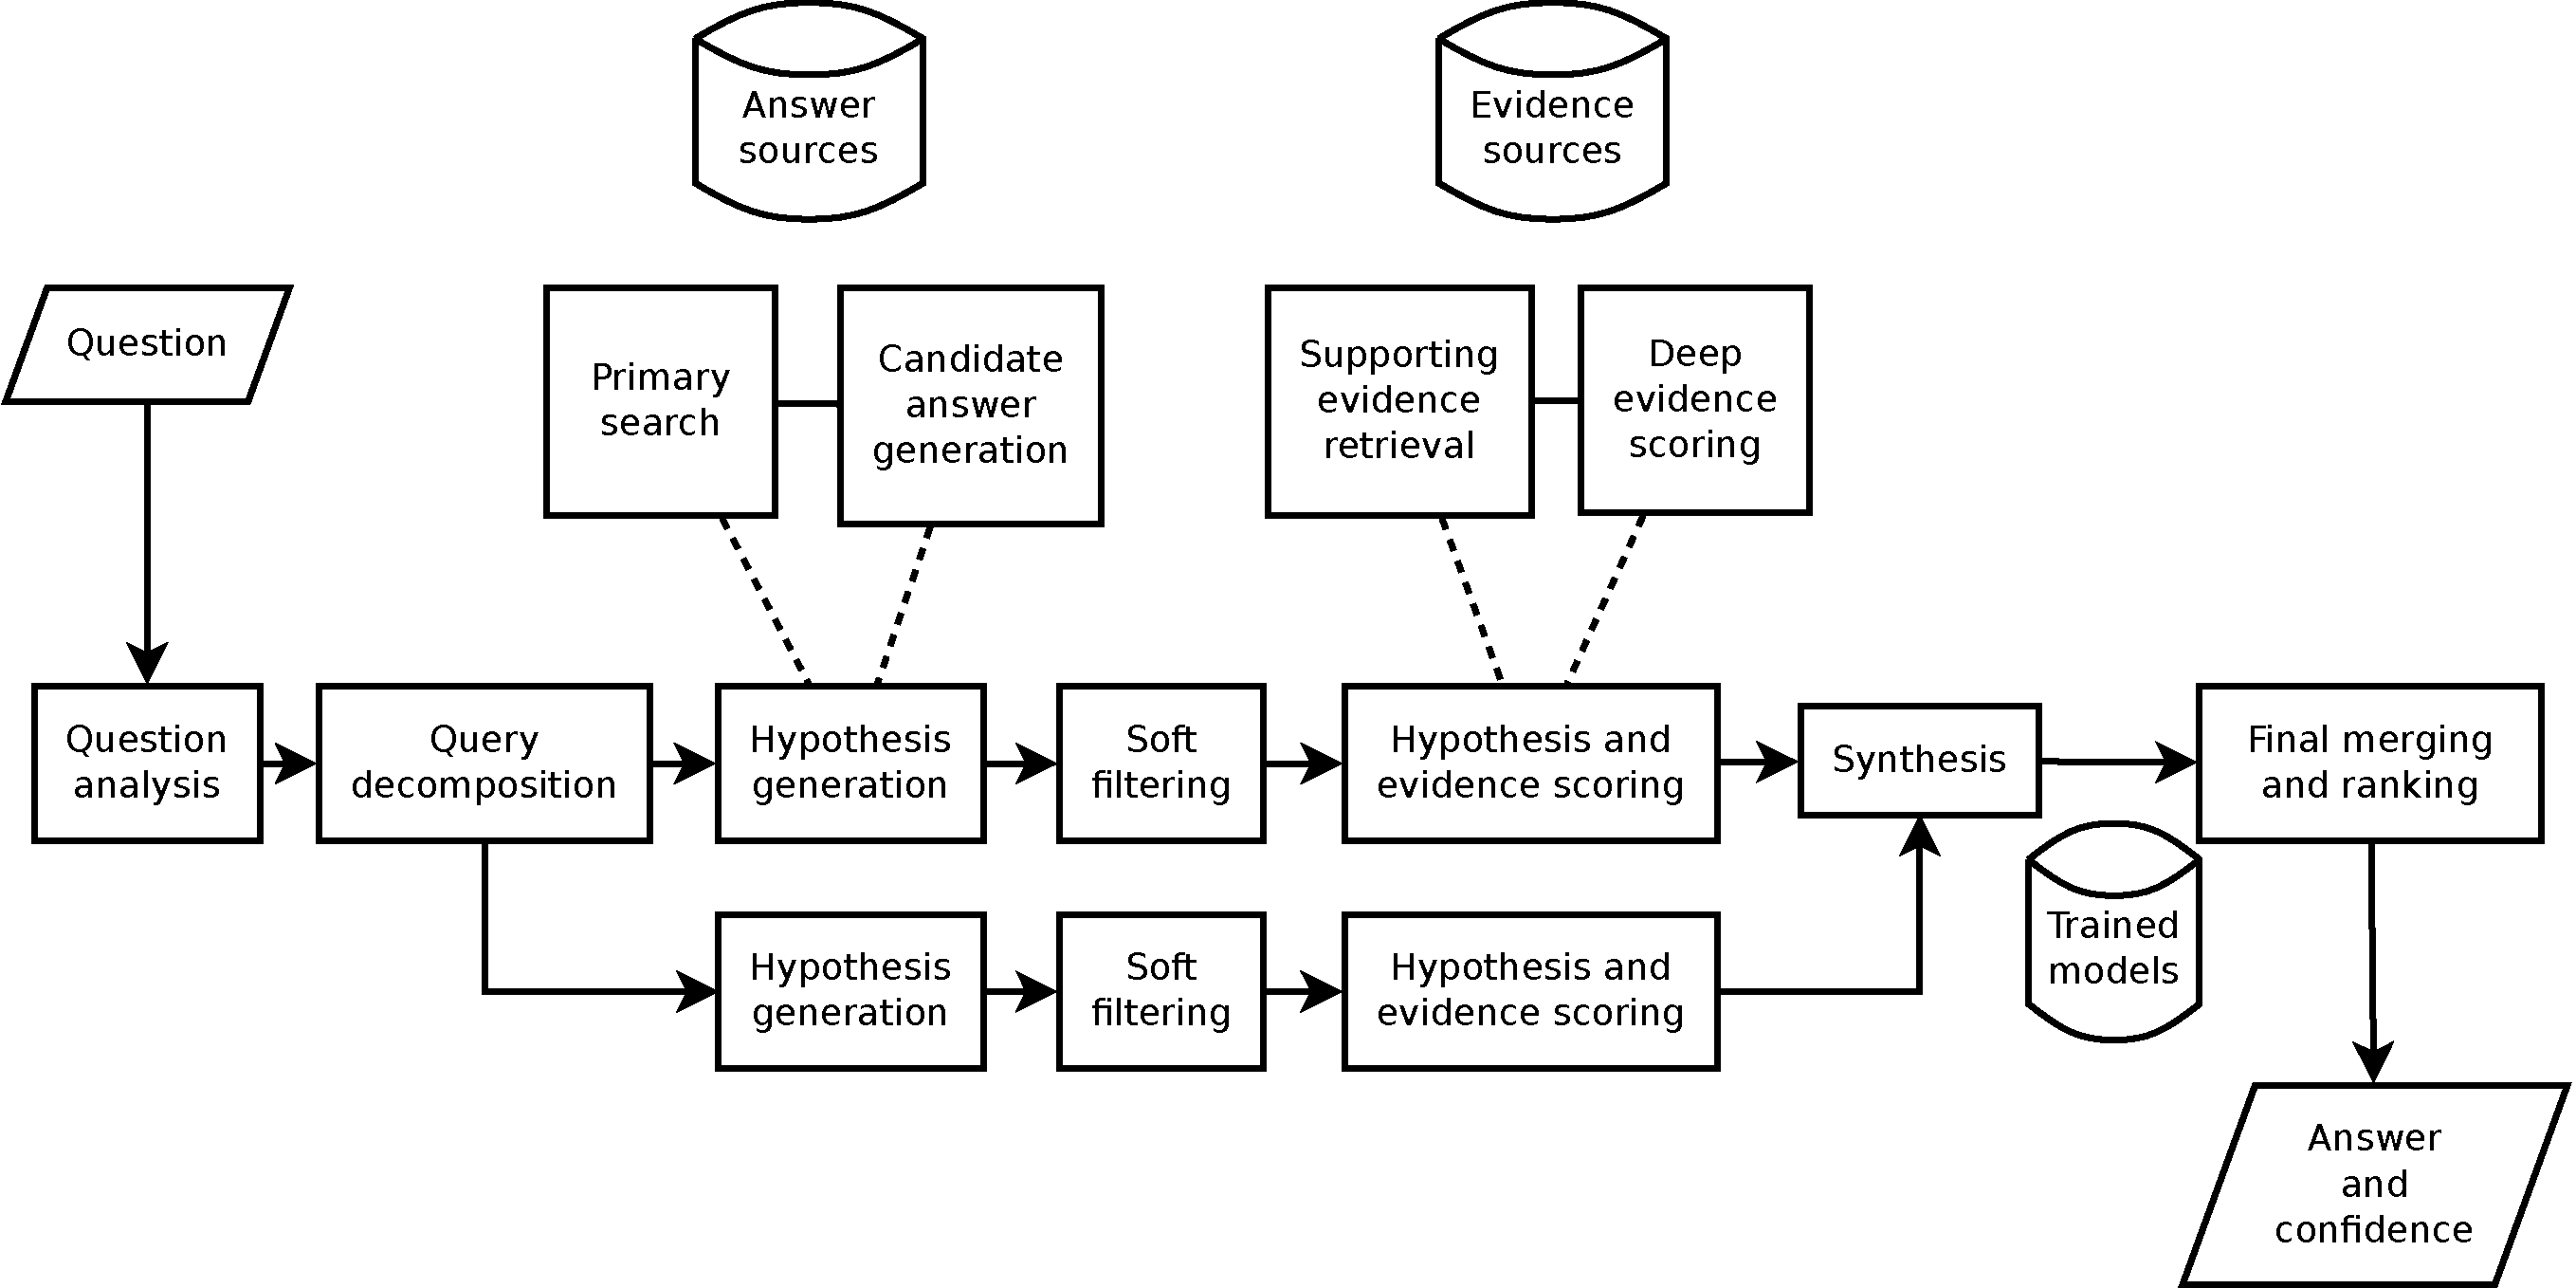
\includegraphics[width=12cm]{Pictures/DeepQA.pdf}
	\caption{Watson's high level architecture}
	\label{ch:rw:ml:watson}
\end{figure}



%----------------------------------------------------------------------------------------
%	DIALOGUE SYSTEMS
%----------------------------------------------------------------------------------------

\section{Dialogue Systems}

Research on dialogue systems has been carried on since the \textbf{early days} of Artificial Intelligence. A milestone in the early work on this field is ELIZA \citep{Weizenbaum:1966:ECP:365153.365168}, which provides the user with a basic human-like interaction based on pattern matching; Figure \ref{ch:rw:ds:ELIZA} shows an instance of these patterns.

Another example is the SHRDLU system \citep{winograd1971procedure}, which interfaces the user with a simple spatial domain by listening to the user's utterances (e.g.\ ``Would you please put the green pyramid in the box?"), and performing actions accordingly in the domain, resolving, if necessary, ambiguous or implicit references to the entities in it.

\begin{figure}
\begin{Verbatim}[frame=single]
["dream", 3, [
 ["*", [
     "What does that dream suggest to you ?",
     "Do you dream often ?",
     "What persons appear in your dreams ?",
     "Do you believe that dreams have something to do
      with your problem ?"
  ]]
]]
\end{Verbatim}
\caption{One of the patterns included in ELIZA's DOCTOR script. It simply tells the system that the user input can be answered with any of the given sentences, whenever it contains the word ``dream".}
\label{ch:rw:ds:ELIZA}
\end{figure}

\subsection{Task vs Nontaks}

According to \cite{Jokinen2009}, modern dialogue systems can be divided in \textbf{two main types}: task-oriented and nontask-oriented. Intuitively, systems in the first category are meant to deal with a specific task such as making a hotel booking, or booking a plane ticket; an example in this category is the MIT Mercury system, a vocal interface to a flight database \citep{Seneff:2000:DMM:1605285.1605288}. On the other hand, nontask-oriented systems are meant to engage in conversations without a specific purpose to fulfill, but the one of delivering a realistic simulation; ELIZA itself is an example of nontask-oriented dialogue system.

Task-oriented systems can be very simple, as simple and well-formalized the task is;  many applications, such as travel service or call routing, can be successfully solved by \textbf{slot-based} systems: each step of the conversation requires some pieces of information, modeled as slots, to be filled in by the user (departure city, arrival city, date, and so on); given the slots to be filled, the dialogue task can be solved with a formal grammar of interaction. As the complexity increases, more phenomena of human interaction have to be modeled, such as turn-taking, multimodality or grounding
%\ignore{CITE RAQUEL'S CHAPTER}
, as well as semantic structures such as quantification and negation; slot-based systems are not sufficient to model these scenarios \citep{Gabsdil03clarificationin}, that require more advanced frameworks such a the Information State Update (ISU) one, which will be tackled in \ref{ch:rw:ds:isu}.

\subsection{Information State Update Dialogue Management}\label{ch:rw:ds:isu}
The ISU approach to Dialogue Management, as it is described by \cite{TraumLarsson03p325}, can be seen as an attempt to reduce the gap between ``theories of dialogue that linguists or philosophers of language may devise and theories directly implemented in dialogue systems".

The linguistic and philosophical roots of this theory can be found in the notion of \textbf{common ground}, as it is defined by [STALNAKER CITE]; on Stalnaker's account, the common ground consists of an unstrucrured set of all the possible worlds that are compatible with the propositions asserted so far in the dialogue. A slightly more sophisticated formulation of the same concept comes from [LEWIS, CITE], who, drawing a parallel between dialogues and baseball, introduces the notion of ``conversational scoreboard", to keep track of the participants' moves. Even closer to the model of Traum and Larsson is \textbf{Ginzburg's dialogue gameboard} [CITATION]; one of the main differences between this model and the other two is represented by the inner structure of the scoreboard, which in Ginzburg is not just a set of propositions, but rather provides a structure made of facts, questions under discussion (QUD) and moves.

Traum and Larsson's notion of \textbf{Information State} takes Ginzburg's DGB one step further, by extending it with a formal representation of what Ginzburg calls the unpublished part of a dialogue partner's mental state (UNPUB-MS), and that will become the private part of the Information State. Figure \ref{ch:rw:ds:isu:ibisis} shows a simple Information State type, as it is implemented in the IBiS1 system \citep[p. 36]{Larsson02issue-baseddialogue}. It can be easily noticed that the IS is split in two sections, ``Private" and ``Shared", each of them containing formal representations of informational components: an agenda of actions being executed, a plan for future actions and a set of beliefs for the \textbf{private} part, the set of propositions in the common ground, a stack of questions under discussion, and the last utterance in the \textbf{shared} part.

The central concept of ISU-based systems is to \textbf{update} this, initially empty, Information State, according to the dialogue moves performed by the DPs. A \textbf{dialogue move} is tipycally a natural language utterance, but, in more complex systems, can also be a different form of interaction, like a gesture. The system detects this interactions, and is able to modify the IS accordingly (e.g.\ inserting a new question under discussion, or marking an action as completed, and so on) thanks to a set of \textbf{update rules}, and an \textbf{update strategy}, to decide on which rules to apply when more than one can be selected.

\begin{figure}
	\centering
	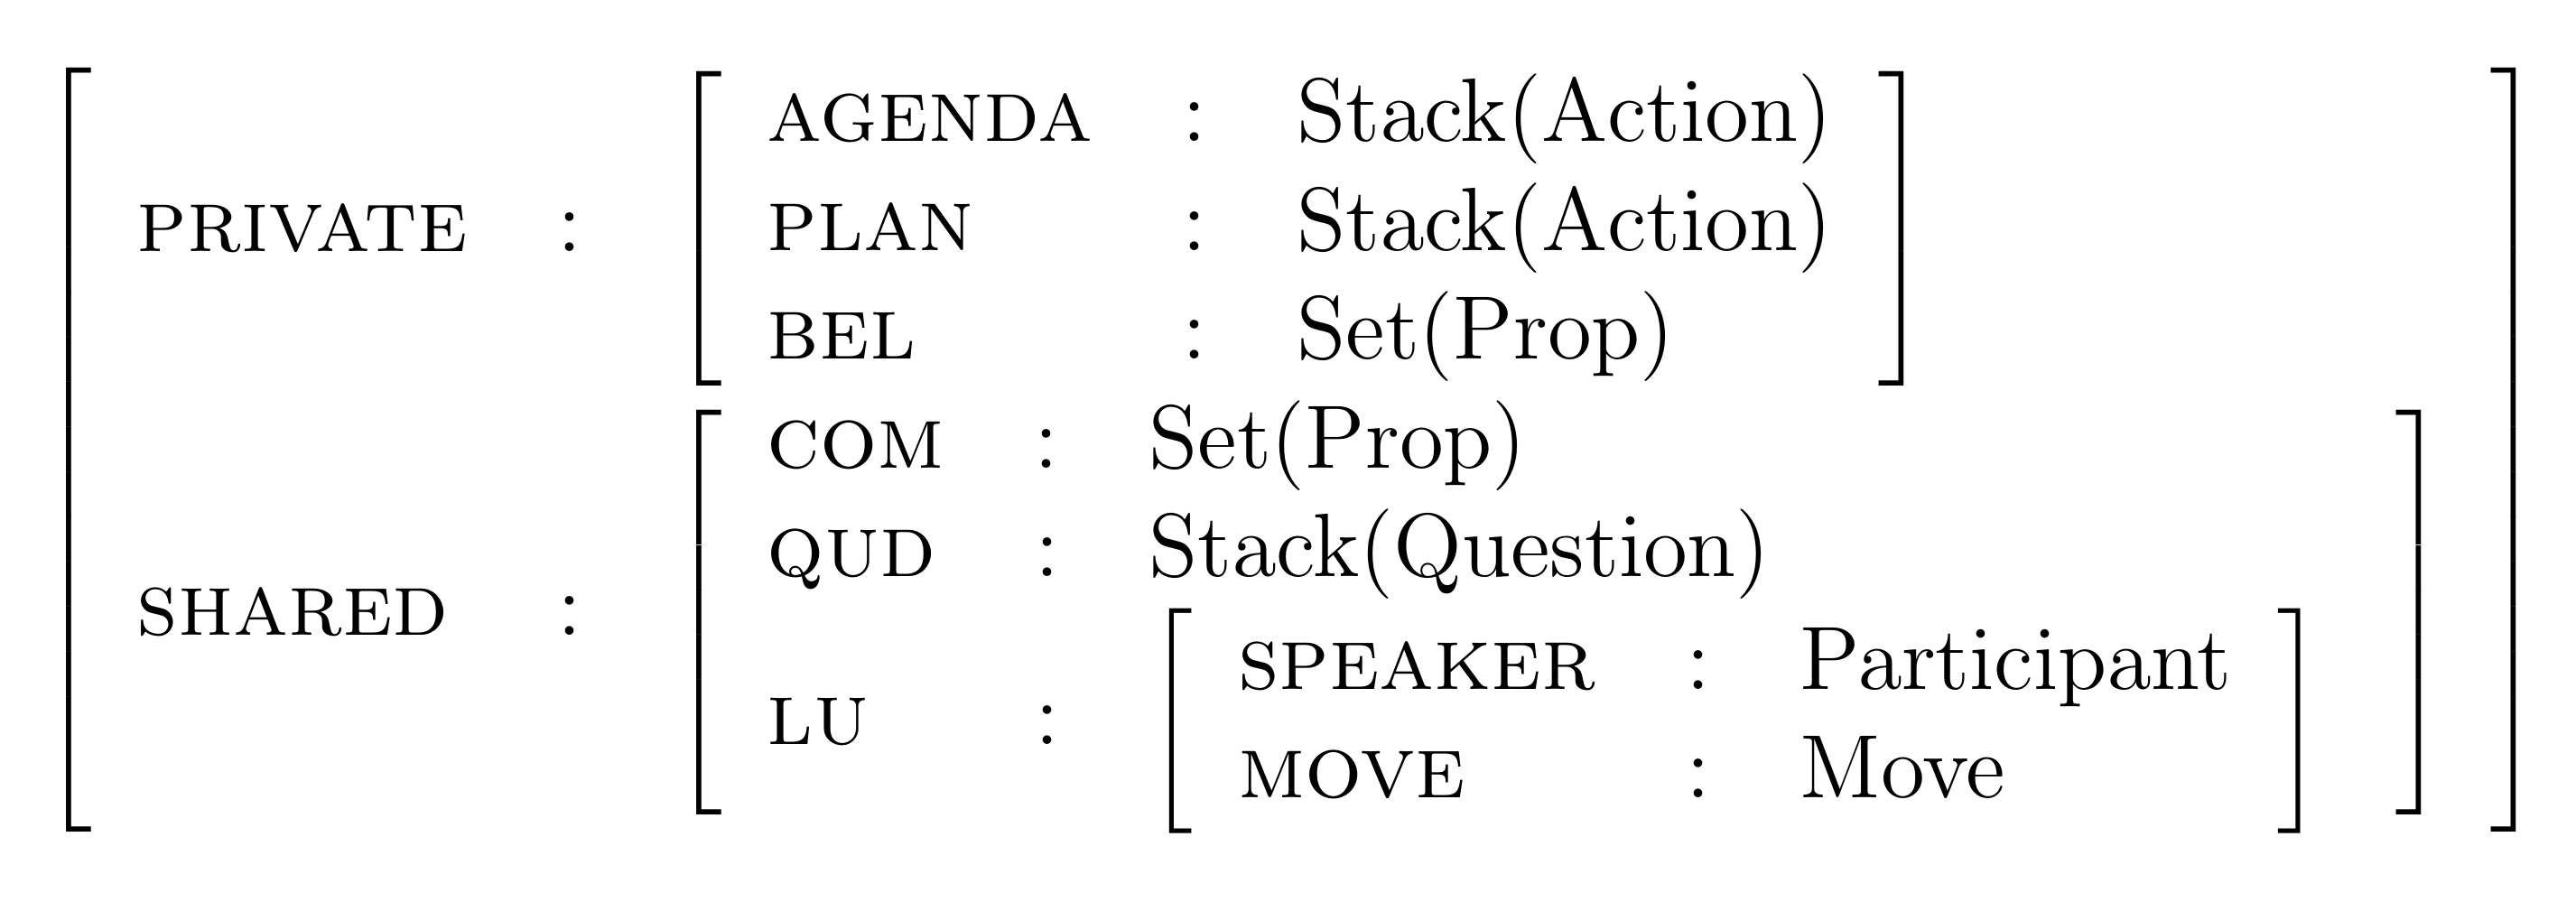
\includegraphics{Pictures/ibis1_is.png}
	\caption{Information State, as it is implemented in IBiS1}
	\label{ch:rw:ds:isu:ibisis}
\end{figure}

This work is relevant to us, as our software builds on the TDM dialogue management library (see \ref{ch:arch:TDM}), which implements the Information State Update framework.
% Chapter Template

\chapter{Architecture} % Main chapter title

\label{ch:arch} % Change X to a consecutive number; for referencing this chapter elsewhere, use \ref{ChapterX}

\lhead{Chapter \ref{ch:arch}. \emph{Architecture}} % Change X to a consecutive number; this is for the header on each page - perhaps a shortened title

%----------------------------------------------------------------------------------------
%	INTRO TEXT
%----------------------------------------------------------------------------------------

The outcome of this thesis project is \pname, a music player application that accepts English utterances as commands, adapts to utterances it has never been exposed to, and learns from them, thus expanding its initial knowledge of the language. The application has been written in Python 2.7, and consists of a client application for the existing OpenTDM dialogue management library. Such a library supports basic dialogue management based on the Information State Update approach, but has no support for grounding or flexible understanding of unknown sentences. Therefore, TDM has been extended with the Language Unit module, that introduces these capabilities.

Section \ref{ch:arch:client} describes the \pname client, Section \ref{ch:arch:TDM} describes the OpenTDM library, and Section \ref{ch:arch:LU} describes the Language Unit module.


%----------------------------------------------------------------------------------------
%	CLIENT
%----------------------------------------------------------------------------------------

\section{The client application} \label{ch:arch:client}
\pname is a client application for the OpenTDM library. An OpenTDM application can be seen as a container for domain-specific \textbf{parameters} for the dialogue manager. These parameters consist of:
\begin{itemize}
\item A \textbf{device} class, containing variables and methods that directly control the actions of the application. The \textit{device} file of a music player application will contain, for instance, variables holding the current playlist, or the current volume level, and methods to play/stop the music, lookup for a song and so forth.
\item An \textbf{ontology}, which main purpose is to define predicates an actions that will be used at dialogue management level. In the case of \pname, an example of predicate is \texttt{current\_song(X)}, that identifies the song currently being played (note that such a predicate must be mirrored in the device file as a variable\footnote{The actual implementation consists of an inner \texttt{current\_song} class of the device class, which access the proper, private, variable of the device file through a \texttt{perform()} method. The reasons that led to such an implementative choice were not made known by the authors of OpenTDM.}); an example of action is \texttt{increase\_volume} that, intuitively, identifies the action of increasing the volume (actions are mirrored as well in the device class, in the same way predicates are).
\item A \textbf{domain} file, which main purpose is to contain the list of plans that will control the dialogue episodes. For instance, the TOP plan of an application is to find out what the user wants to do. Another example of a plan in \pname is the \texttt{increase\_volume} plan: step 1 of the plan is ask the user for how much the volume should be increased, step 2 is to perform the actual action through the device.
\item A \textbf{grammar} implemented using the Grammatical Framework\footnote{http://www.grammaticalframework.org/}. This part will not be discussed, since, as it is explained in Section \ref{ch:arch:LU}, the Grammatical Framework in OpenTDM has been replaced with a specifically created module called Language Unit.
\end{itemize}

The dialogue management logic is left to OpenTDM, that will be discussed in the next section.


%----------------------------------------------------------------------------------------
%	TDM
%----------------------------------------------------------------------------------------

\section{OpenTDM} \label{ch:arch:TDM}
OpenTDM is a dialogue management library developed and maintained by Talkmatic\footnote{http://talkamatic.se/} based on the Information State Update framework

\ldots

%----------------------------------------------------------------------------------------
%	LU
%----------------------------------------------------------------------------------------
\section{The Language Unit} \label{ch:arch:LU}
The Language Unit (LU) is a Python library that have been specifically created to support \pname. The purpose of this library is to perform the classification task as it has been defined so far.

\subsection{Language}
The \texttt{Language} class is the main class of LU, its purpose is to model a natural language under the following abstraction: a Language is defined by a finite set of Meanings (labels); a Meaning is defined by a finite set of Sentences expressing that Meaning. As an example, the \pname language consists of a number of meanings, each of them defining an action for the application to perform; one of this meaning can be the one to pause the current song; this meaning will be realized by a number of English sentences, like ``Pause the song", ``Suspend the music", or ``Pause the current track". For the purpose of language understanding, a Sentence can be brougth down to any of its (linguistic or non-linguistic) constituents called Chunks or Phrases. A chunk is formed by one or more Words.

The following are the main capabilities implemented in the Language class:
\begin{itemize}
\item \textbf{Load} and \textbf{save} languages. Each OpenTDM application must define a \texttt{language/} folder where the language is stored, in the form of a \texttt{.l} file. Such a file is just a dump of all the meanings and their example sentences. Since the language  can evolve through learning, applications' language files are updated every time the application is run and dialogue interactions are performed.
\item \textbf{Learn} a sentence. When a new labeled example (a sentence with its meaning label) is provided, the knowledge of the language is extended. This is done adding the new sentence to the list of sentences realizing that meaning, and drawing statistics (e.g. the frequency of a certain word/phrase in the given meaning) to improve the model of the meaning. Note that, when a language is loaded for the first time, every sentence in it is run through the learning procedure to initialize the statistics.
\item \textbf{Understand} an input sentence. The core task of the Language Unit is associate an input sentence to its correct meaning. While this operation is trivial when the input sentence is already present in the language, it becomes hard for unknown examples. In this latter case the LU computes a score for the sentence against each of the meanings that are present in the language; the meaning that achieves the best score is given as an output, along with the score itself, representing the degree of confidence for the output to be correct. The way sentences are scored is presented in the next section.
\end{itemize}

\subsection{Scores}

\subsubsection{Meaning Score}

\subsubsection{Sentence Score}

\subsubsection{Chunk Score}
Chunks are compared using the M2 algorithm, that is explained in detail in Chapter \ref{ch:M2}.

\subsubsection{Word Score}
Word scores are as well explained in Chapter \ref{ch:M2}.

\subsection{Machine Learning}


\ldots
 

\chapter{Sentence similarity computation} % Main chapter title

\label{ch:M2} % Change X to a consecutive number; for referencing this chapter elsewhere, use \ref{ChapterX}

\lhead{Chapter \ref{ch:M2}. \emph{The M2 matching algorithm}} % Change X to a consecutive number; this is for the header on each page - perhaps a shortened title

In the context of sentences \textbf{classification}, where the task is to label an unknown input sentence with the correct meaning, and each meaning is defined by a set of representative natural language sentences (as it was defined in the Introduction), one crucial point is to measure the similarity of the input sentence with each of the sentences defining each meaning.

Computing a \textbf{similarity score} between two natural language \textbf{sentences} is not a trivial problem. Many features can be taken into account to solve it, such as the syntactic structure of the sentence, or the meaning of the single words, or their order; all of these features are informative respect to the meaning of the sentence, and it is reasonable to assume they are all considered by humans solving the same task. Here we describe a recursive, dynamic programming \textbf{algorithm} for sentence comparison aimed to exploit word-based information, as well as the syntactic one, expressed in the form of unsupervised learned binary trees.

% A bit more on literature, relation to the work would be nice..

The algorithm presented in this thesis aims to provide a similarity measure for two sentences $s_1$ and $s_2$ featuring many of the ideas that have proven to be successful in recent developments of Computational Linguistics. The following are some of the key insights of the algorithm:

\begin{itemize}
\item \textbf{Every possible} sub-sentence of $s_1$ is compared with every possible sub-sentence of $s_2$.
\item A score between two chunks of text is build \textbf{recursively} on the best matches of smaller chunks, and always brought down to scores between single words.
\item \textbf{Dynamic programming} is used to increase the efficiency of the algorithm, preventing it from computing the same result two times.
\item Other than the similarity score, the algorithm outputs the most probable chunking of each sentence in the form of an unlabeled binary \textbf{parse tree}.
\item Other than the similarity score and the parse trees, the algorithm outputs the most likely \textbf{alignment} between the chunks of the two sentences.
\item Every score is expressed as a linear combination of \textbf{features}, designed to be independent and extensible.
\item The partial computations of the algorithm can be stored and further used to implement a learning model.
\end{itemize}

%Document structure
This chapter is \textbf{structured} as follows. Section \ref{algo} describes the algorithm theoretically. %and in a better world a complexity analysis
%Section \ref{example} walks through a toy example.
Section \ref{learning} describes possible extensions and improvements. Section \ref{conclusions} draws the conclusion of the paper.

\section{The M2 Matching Algorithm} \label{algo}
\begin{algorithm}
  \SetKwData{Left}{left}
  \SetKwData{Up}{up}
  \SetKwFunction{WWScore}{$\tau$}
  \SetKwFunction{CCScore}{$\tilde{\sigma}$}
  \SetKwFunction{Length}{Length}
  \SetKwFunction{Split}{Split}
  \SetKwFunction{Set}{Set}
  \SetKwFunction{Append}{Append}
  \SetKwFunction{Max}{Max}
  \SetKwInOut{Input}{input}
  \SetKwInOut{Output}{output}
  \SetKw{In}{in}

\Indm  
  \Input{$c_1,c_2$ chunks of text; $T$ partial results table}
  \Output{$\sigma(c_1,c_2)$ Similarity score between $c_1$ e $c_2$}
\Indp
  \BlankLine
  \uIf{c1,c2 are words}{ \label{main:bc1}
	  \Return{\WWScore{$c_1,c_2$} \label{main:bc2} }
  }
  \BlankLine
  $S\leftarrow[\ ]$\; \label{main:cinit}
  \For{$i\leftarrow 1$ \KwTo \Length{$c_1$}}{ \label{main:loopi}
    $C_1 \leftarrow $ \Split{$c_1$,i}\; \label{main:spliti}
		\For{$j\leftarrow 1$ \KwTo \Length{$c_2$}}{ \label{main:loopj}
		\lIf{i=\Length{$c_1$} and j=\Length{$c_2$}}{break} \label{main:break}
		\BlankLine
		$C_2 \leftarrow $ \Split{$c_2$,j}\; \label{main:splitj}
		\BlankLine
		\ForEach{$sc_1$ \In $C_1$}{ \label{main:fe1}
			\ForEach{$sc_2$ \In $C_2$}{ \label{main:fe2}
				\uIf{$T[sc_1,sc_2]=\emptyset$}{$T[sc_1,sc_2] \leftarrow \sigma(sc_1,sc_2,T)$ \label{main:tabass} \label{main:tupdate}}
			}
		}
		\BlankLine
		\Append{$S$,\CCScore{$C_1,C_2,T$}} \label{main:cappend}
 }
	}
	\BlankLine
	\Return \Max{$R$} \label{main:return}
\caption{The main algorithm\label{main}}
\end{algorithm}

Algorithm \ref{main} contains the main loop of the sentence scoring algorithm. Before entering the details of it, it is necessary to say that:
\begin{itemize}
\item The input $c_1,c_2$ can be any \textbf{chunks} of text because, while the algorithm is called with two sentences in input, it will recursively call itself on every possible chunk extracted from the two sentences.
\item The input $T$ (T for Table) is a data structure holding the intermediate results of the algorithm. As we can infer from line \ref{main:tabass} of Algorithm \ref{main}, $T[c_1,c_2]=\sigma(c_1,c_2)$
\item $\tau(c_1,c_2)$ returns a similarity score between two words. This score is a linear combination of independent features. At the moment, the following features are taken into account:
\begin{itemize}
\item Equality (boolean) -- 1 if $c_1=c_2$, 0 otherwise
\item Edit distance -- $1-d$, where $d$ is the Levelshtein distance \citep{levelshtein-66-binary} between $c_1$ and $c_2$, as it is implemented in NLTK \citep{Loper:2002:NNL:1118108.1118117}
\item Difference in position -- $(1/|p_{c_1}-p_{c_2}|)^\alpha$, where $p_{c_i}$ is the position of $c_i$ in the sentence, and $\alpha$ is a free parameter.
\item Wordnet \citep{Miller:1995:WLD:219717.219748} Path Length similarity, as it is implemented in NLTK
\end{itemize}
The weights of the single features, now static, are meant to be trained through Machine Learning
\item \texttt{Length($c$)} returns the number of words contained in the chunk $c$
\item \texttt{Split($c,i$)} returns a list of two chunks, one containing the words of $c$ from the first to the $i$th, and the other containing the words of $c$ form the $(i+1)$th to the last.

If the $i$th word is the last word of $c$, it returns a list containing the only element $c$.
\item \texttt{Append($L,x$)} is the standard \emph{append} operation for lists, adding the element $x$ in the last position of the list $L$.
\item $\hat{\sigma}(C_1,C_2,T)$ returns the score of $c_1,c_2$ \textbf{given} a particular 2-split of the two chunks. Such a score is computed combining the ones of the smaller constituents of $c_1,c_2$, which are required to be already present in the table T.

The score is again the linear combination of independent features, leaving its implementation open and extensible.

At the moment the only feature being employed is the average of the scores of the best alignments of the sub-chunks in $C_1$ with the ones in $C_2$.

For example, given $C_1=[\text{``increase",``the volume"}]$ and $C_2=[\text{``raise"},\\ \text{``the volume"}]$, ``increase" is likely to achieve the best score with ``raise" (eg. $T[\text{``increase",``raise"}]=0.8$), as well as ``the volume" will be aligned with ``the volume" ($T[\text{``the volume",``the volume"}]=1$)). The score of ``increase the volume" and ``raise the volume", in this particular splitting, will thus be the average of the two, 0.9.
\end{itemize}
After these premises it is relatively easy to walk through the pseudo-code of Algorithm \ref{main}. Lines \ref{main:bc1} and \ref{main:bc2} handle the base case, that is, when the algorithm is run on \textbf{two words}; in this case the result of the Word Similarity function, which is described above, is returned.

At line \ref{main:cinit} the list of \textbf{candidate results} is initialized as an empty list. This is because more than one score will be computed for $c_1$ and $c_2$, the maximum of which will be returned as a result.

Lines \ref{main:loopi} and \ref{main:loopj} define a nested loop structure, which purpose is to update the two indexes $i$ (from the first to the last word of $c_1$) and $j$ (from the first to the last word of $c_2$) to cover \textbf{every possible combination} of word positions in the two input strings. These indexes are used to \textbf{split} the input chunks in smaller parts (lines \ref{main:spliti} and \ref{main:splitj}). As an example, if the input is given by $c_1=$``increase the volume", $c_2=$``raise the volume", the outer loop will produce the three possible values of $C_1$: [``increase",``the volume"], [``increase the",``volume"] and [``increase the volume"]; each of these values will be combined, in the inner loop, with the three possible values of $C_2$: [``raise",``the volume"], [``raise the",``volume"] and [``raise the volume"].

Note that, while it is reasonable to consider the entire $c_1$ and $c_2$ in the comparisons (eg. if $c_1=$``quit",$c_2=$``quit please", we'd want the whole $c_1$ to be associated with the ``quit" sub-part of $c_2$), it is necessary to prevent the two entire $c_1$ and $c_2$ to be associated at the same time, thus producing an \textbf{infinite loop}; this is done in line \ref{main:break}.

The next part of the inner loop, from line \ref{main:fe1} to line \ref{main:fe2} combines every sub-chunk of $c_1$ ($sc_1 \in C_1$) with every sub-chunk of $c_2$ ($sc_2 \in C_2$); note that $C_1$ and $C_2$ contain either one or two elements. Every combination that is not present in the table is scored with a \textbf{recursive} call to the algorithm itself, and the resulting score is saved in the table (line \ref{main:tupdate}).

The last operation done in the loop, at line \ref{main:cappend}, is to combine the sub-scores that have just been scored in the table to compute the final score of this particular subdivision of $c_1$ and $c_2$. This is a \textbf{candidate score} for $c_1$ and $c_2$, and thus is appended to the list of candidate scores. As we already said, the definition of this combination is open; however it is most reasonable for the $\hat{\sigma}$ function to find the \textbf{best alignment} between the input sub-chunks, and provide a score based on it. It is clear that the definition of $\hat{\sigma}$ is crucial for getting sensible results from the algorithm. Furthermore, $\hat{\sigma}$ is the point where the algorithm can be extended with Machine Learning capabilities, that will be discussed in Section \ref{learning}.

At line \ref{main:return} the function returns the \textbf{maximum of the candidate} score, that is, the split that produced the best score (eg. for ``increase the volume" vs ``raise the volume", the score of ``increase $\vert$ the volume" vs ``raise $\vert$ the volume" is likely to produce a better score than ``increase $\vert$ the volume" vs. ``raise the $\vert$ volume"). Note that this decision determines the branching of one level of the recursion tree; once the algorithm is done computing the score between two sentences, a traceback of the selected splits can be interpreted as a parse tree for the two input sentences.

%\section{An Example} \label{example}

\section{Machine Learning Possibilities} \label{learning}
The basic algorithm described in section \ref{algo} only deals with \textbf{static features} to measure similarities: the score of two words is derived from equality, edit distance, Wordnet path length and so on; the score of chunks is the average of the scores of the best alignments of their components.

In this section I address the question whether it is possible, and how, for the algorithm to \textbf{learn} from the sentences it is parsing. In other words, given a sentence of which I know the meaning, how can I use this information to improve the way I process new sentences?

Here I consider \textbf{three features} based on Statistical Language Processing methods to address this problem: chunk likelihood, class-conditional chunk weight and alignments likelihood.

\subsection{Chunk Likelihood} \label{ch3:ml:cl}
% Relative frequency across all sentences
% Used to select good chunks
Let's consider the following pair of sentences:
%\begin{quote}
\enumsentence{Pump up the volume} %\\
\enumsentence{Turn up the volume}
%\end{quote}

As an English-speaking human being I immediately associate the phrase ``pump up" with ``turn up" and ``the volume" with its analogue. One of the reasons I make this association rather than, for instance, associating ``pump" with ``turn" and ``up the volume" with its analogue, is that I have good experience of the phrase ``the volume" being used in different contexts, while fewer times I encounter ``up the volume".

Thus a feature that can be useful to \textbf{enforce good chunking} of the input sentences is the likelihood of a chunk of text (where a chunk is defined as either a word or a combination of chunks). This feature can be modeled as the relative count of each chunk in the whole pool of the ones that have been recorded:
$$
l(c)=\frac{\text{\# of }c}{\text{\# of total chunks}}
$$

Note that this feature is completely unsupervised, in that it does not require a Meaning label to be computed.
\subsection{Class-conditional Chunk Weight} \label{ch3:ml:cc}
% frequency in class / frequency overall
% Used to weight more chunks that are representative for one class
Let's consider the following three sentences:
%\begin{quote}
\enumsentence{Increase the volume} %\\
\enumsentence{I would appreciate if you could increase a bit the the volume} %\\
\enumsentence{Decrease the volume}
%\end{quote}

With a reasonable approximation, the first two sentences have the same meaning, while the last says the opposite, although the first and the last sentence are much more similar from a syntactic point of view. Nevertheless, no English speaker would bother wondering about hidden meanings behind phrases like ``I would appreciate", or ``if you could": everyone could tell that the second sentence is no more than the first one, with some more formal dressing.

Especially, when I listen to the second sentence, I can immediately locate ``increase" and ``the volume" as the most informative phrases, while filtering out the rest as less relevant. One of the reasons I am able to do this is that I have memory of ``I would appreciate if you could" used in sentences conveying lots of different meanings, while ``increase" is likely to appear only in situations where something is increased.

A feature that could be useful to spot the \textbf{informativeness} of chunks can be the conditional probability of the chunk, given a certain meaning:
$$
l(c|m)=\frac{\text{\# of }c\text{ in }m}{\text{\# of }c}
$$

This feature can be used to weight the score of different chunks in the sentence, so for more informative chunks to influence more of the total score mass.
%l(c|m,M)?
\subsection{Alignment Likelihood}\label{ch3:ml:al}
% Recursive score of alignments
% Used to align chunks correctly
Let's consider the following pair of sentences:
%\begin{quote}
\enumsentence{Skip this track} %\\
\enumsentence{Jump over this song}
%\end{quote}
Again, English speakers can easily associate the meaning of ``skip" with the one of ``jump over", and the meaning of ``track" with the one of ``song".

One device that the algorithm uses to solve this problem is the \textbf{Wordnet} Path Lenght measure for word comparison. However, it has been noticed that this measure has its limits. In particular
\begin{itemize}
\item Not all the words are included in Wordnet
\item Being a static measure, it cannot be adapted to the domain
\item It has difficulties spotting antonyms
\end{itemize}
The alignment likelihood measure can be used to \textbf{enforce correct alignments} of different chunks.
$$
l(c_2|c_1)=\frac{\text{\# of }c_1-c_2\text{ alignments }}{\text{\# of }c_1\text{ alignments}}
$$
Note that, since no alignment labels are provided in the dataset (each sentence is labeled with a meaning, but its syntactic structure is hidden), this measure have to be trained in an unsupervised fashion. This problem shares a lot with the alignment likelihood in \textbf{Machine Translation}, even though here we can take advantage of the chunks sharing the same language (thus allowing some clever initialization of unsupervised methods with sensible guesses based, for instance, on Wordnet). On the other side our problem presents less precise training data, in that, while MT alignments are trained on sentence pairs, here we have a group of sentences sharing a same meaning; it can be argued that this cannot allow for strong syntactic assumptions.
% MT: T: more similar syntactic structure (label sentence by sentence)

\section{Summary} \label{conclusions}
In this chapter we described an algorithm to compare the similarity of two input sentences. Its main \textbf{advantages} are the concurrent consideration of many features like word meanings, position and overlapping, as well as the structure of the sentences, having the result in the form of aligned binary trees. The algorithm is recursive and exhaustive in that considers all the possible alignments of all the possible combinations of all the possible binary trees of the two input sentences, maximizing the efficiency with dynamic programming. Due to its modular structure, the algorithm can be easily extended with new features, allowing its integration with well-known Machine Learning techniques in Computational Linguistics (eg. Expectation-Maximization for computing word/phrase alignment probabilities).

There are some assumptions and \textbf{weak points} as well. First of all, the algorithm is inherently binary, in that every recursion step is made of a 2-split of the two input strings; this may have an effect in the way partial scores are combined. More generally, this ``two times binary" recursive structure makes the features design task hard, since the effect of one operation is not easy to control over a potentially unlimited number of recursion steps. Also the number of parameters can become high, since each score is a linear combination of single features, requiring a separate Machine Learning training.

Lastly, this paper only describes the \textbf{backbone} of the algorithm, which is not yet ready for more formal tests on existing corpora. The main steps ahead before expecting good results from it include a better tuning and possible extension of the existing features  and the implementation of Machine Learning techniques to include alignment probabilities and more advanced statistical features for the chunks being compared (eg. their degree of informativeness).

%\begin{thebibliography}{9}

%\bibitem{achananuparp08}
%Palakorn Achananuparp, Xiaohua Hu, Xiajiong Shen. The Evaluation of Sentence Similarity Measures. Lecture Notes in Computer Science Volume 5182, 2008, pp 305-316

%\bibitem{udop}
%Rens Bod. Unsupervised parsing with U-DOP. CoNLL-X '06 Proceedings of the Tenth Conference on Computational Natural Language Learning, 2006, pp 85-92. 

%\bibitem{ibmmt}
%P. Brown, S. Della Pietra, V. Della Pietra, and R. Mercer (1993). The mathematics of statistical machine translation: parameter estimation. Computational Linguistics, 19(2), 263-311.

%\end{thebibliography}

% Chapter Template

\chapter{Interaction} % Main chapter title

\label{ch:interaction} % Change X to a consecutive number; for referencing this chapter elsewhere, use \ref{ChapterX}

\lhead{Chapter \ref{ch:interaction}. \emph{Interaction}} % Change X to a consecutive number; this is for the header on each page - perhaps a shortened title

%----------------------------------------------------------------------------------------
%	INTRO TEXT
%----------------------------------------------------------------------------------------
This chapter describes how the \pname software is able to exploit the information contained into an unknown input sentence, to make \textbf{pertinent questions} to the user about the meaning of its single components, and learn from the interaction. 

%----------------------------------------------------------------------------------------
%	MINIMAL AMBIGUOUS FRAGMENT
%----------------------------------------------------------------------------------------

\section{Ambiguous fragments location}

\ldots software looking for minimal ambiguous fragments in the input sentence to ask questions about\ldots

%----------------------------------------------------------------------------------------
%	INTERACTION EPISODE
%----------------------------------------------------------------------------------------

\section{Production of the interaction episode}

\ldots generation of the questions and storage of the answers\ldots

%----------------------------------------------------------------------------------------
%	KNOWLEDGE UPDATE
%----------------------------------------------------------------------------------------

\section{Knowledge update}

\ldots update of the database\ldots
 
%\input{./Chapters/Chapter5} 
...
-future/open questions
 - Machine Learning on weights
 - maybe dynamic weights (eg. disregard other Word features if Equals=1)
 - Tabu game to get corpus
 - Weighting of sources (use confidence of sentences)
 - Better integration with OpenTDM (requires documentation)
 - Meta-learning of episodes (eg. new ways to do disambiguation interactions)
 
%\input{./Chapters/Chapter7}

%----------------------------------------------------------------------------------------
%	THESIS CONTENT - APPENDICES
%----------------------------------------------------------------------------------------

\addtocontents{toc}{\vspace{2em}} % Add a gap in the Contents, for aesthetics

\appendix % Cue to tell LaTeX that the following 'chapters' are Appendices

% Include the appendices of the thesis as separate files from the Appendices folder
% Uncomment the lines as you write the Appendices

% Appendix A

\chapter{An Information State Update Example} % Main appendix title

\label{a:isu} % For referencing this appendix elsewhere, use \ref{isu}

\lhead{Appendix A. \emph{An Information State Update Example}} % This is for the header on each page - perhaps a shortened title

This appendix shows how SVPlay's Information State (IS) is updated during a \textbf{simple user interaction}, where the latter asks for the current song title. The interaction, at input/output level, is the following:
\begin{verbatim}
S> How can I help you?
U> what is the current song  
S> It's All Over Now, by The Rolling Stones
\end{verbatim}

As a premise, it is necessary to point out that, as OpenTDM comes with \textbf{no documentation}, the information contained in this appendix was derived from our analysis of the software's source code and log files. For this reason, it is possible that our explanation will not cover some parts of the process, either irrelevant or still obscure.

At t=0 the information state of the application is \textbf{empty}. While for the next steps we will only consider a subset of the OpenTDM's Total Information State (TIS), Figure \ref{a:isu:tis} shows the complete TIS, as it was reconstructed from the application's log. We can immediately spot, in the figure, the two main parts of the IS: private and shared. The most relevant parts of the \textbf{private} are
\begin{itemize}
	\item The list of the system's private \textbf{beliefs} (\texttt{bel})
	\item The stack of \textbf{plan} items that the system will execute.
\end{itemize}

From the \textbf{shared} part of the IS is important to highlight the stack of \textbf{questions under discussion} (\texttt{qud}), representing the issues that user and system will cooperatively try to solve. For the sake of record, we report that the \texttt{lu} field contains the \textit{last utterance} to be pronounced, either by the system or by the user; similarly, \texttt{pm} stands for \textit{previous move}, and \texttt{com} for \textit{common ground}.

\begin{figure}
\centering
$\left[\begin{tabular}{l l}
application &	\texttt{Application(`svplay', <Ontology>, <Domain>)} \\
device\_outputs &	\texttt{stack([])} \\
devices &	\texttt{\{`MplayDevice': <Device>\}} \\
input\_event &	\texttt{Event(START)} \\
latest\_moves & \texttt{open\_queue([`\#'])} \\
latest\_speaker & \texttt{None} \\
next\_utterance & 	$\left[\begin{tabular}{l l}
				alts & \texttt{[]} \\
				context & \texttt{\{\}} \\
				moves & \texttt{open\_queue([`\#'])} \\
				plan\_item & \texttt{None} \\
				\end{tabular}\right]$ \\
output & \  \\
passive\_mode & \texttt{False} \\
PRIVATE &	$\left[\begin{tabular}{l l}
			agenda & \texttt{open\_queue([`\#'])} \\
			bel & \texttt{\{\}} \\
			nim & \texttt{open\_queue([`\#'])} \\
			plan & \texttt{stack([do(top)])} \\
			\end{tabular}\right]$ \\
program\_state & \texttt{RUN} \\
recognised\_utterance & \texttt{None} \\
SHARED &	$\left[\begin{tabular}{l l}
			actions & \texttt{stackset([top])} \\
			com & \texttt{\{\}} \\
			issues & \texttt{stackset([])} \\
			lu &	$\left[\begin{tabular}{l l}
				moves & \texttt{\{\}} \\
				speaker & \texttt{None} \\
				turn\_count & \texttt{\{\}} \\
				\end{tabular}\right]$ \\
			pm & \texttt{\{\}} \\
			previous\_action & \texttt{None} \\
			qud & \texttt{stackset([])} \\
			\end{tabular}\right]$ \\
sys\_truns & 0 \\
timeout & 	$\left[\begin{tabular}{l l}
			duration & \texttt{None} \\
			enabled & \texttt{False} \\
			\end{tabular}\right]$ \\
\end{tabular}\right]$

\caption{An empty Total Information State in OpenTDM}
\label{a:isu:tis}
\end{figure}

We notice that \texttt{Event(START)} is pushed by default in the \texttt{input\_event} fileld (\texttt{application} and \texttt{device\_outputs} are filled as well, but they just hold static information, that will not change during the execution). This is because OpenTDM is \textbf{event-driven}: everything happening in the system is a consequence of an event, and \texttt{START} is the one that starts the causal chain. The complete list of events is defined in the \texttt{maharani.event} module.

As a consequence of the \texttt{START} event. the software will plan his first dialogue move. This is done by pushing the top plan in the \textbf{private plan} section. The top plan is defined in the application ontology;
\begin{verbatim}
["forget_all",
 "findout(?set([issue(?X.current_song(X)), issue(?X.my_name(X)),
	                action(increase_volume)]))"]
\end{verbatim}
This clears all the current believes and raises the issue of determine \textbf{what the user wants to do}. Literally, the \texttt{findout()} statement aims to decide whether the user wants to know the title of the current song, know the system's name or increase the volume. As a matter of fact, \pname supports more than these three actions, but the logic form of the top plan could not be changed accordingly because of the lack of documentation.

This plan has the effect of producing a \texttt{SYSTEM\_MOVES} event, that will prompt the user with the \textbf{question} ``How can I help you?". Note that the surface form of this question will be provided by the Language Unit, and is defined in \texttt{language/<APP><LANG>Prod.py}, in the application directory. Once the question is asked, it can be pushed in the ``questions under discussion" part of the \textbf{shared} IS.

The following is the resulting Information State:

\begin{table}[ht]
\small
$\left[\begin{tabular}{l l}
input\_event &	\texttt{Event(SYSTEM\_MOVES,} \\
\ & \texttt{[(Move(ask(?set([issue(?X.current\_song(X)),} \\
\ & \texttt{\hspace*{11em} issue(?X.my\_name(X)),} \\
\ & \texttt{\hspace*{11em} action(increase\_volume)])),} \\
\ & \texttt{\hspace*{3em} speaker=SYS, modality=speech),} \\
\ & \texttt{\hspace*{3em} `How can I help you?')])} \\
latest\_speaker & \texttt{SYS} \\
PRIVATE &	$\left[\begin{tabular}{l l}
			bel & \texttt{\{\}} \\
			plan & \texttt{stack([findout(?set([issue(?X.current\_song(X)),}\\
\ &			\texttt{\hspace*{5em}issue(?X.my\_name(X)),}\\
\ &			\texttt{\hspace*{5em} action(increase\_volume)]))])} \\
			\end{tabular}\right]$ \\
recognised\_utterance & \texttt{None} \\
SHARED &	$\left[\begin{tabular}{l l}
			com & \texttt{\{\}} \\
			qud & \texttt{stackset([?set([issue(?X.current\_song(X)),}\\
\ &			\texttt{\hspace*{5em}issue(?X.my\_name(X)),}\\
\ &			\texttt{\hspace*{5em} action(increase\_volume)]))])} \\
			\end{tabular}\right]$ \\
\end{tabular}\right]$
\end{table}

At this point, the \textbf{user} inputs the sentence ``What is the current song". This input is given to the language unit, that will return its formal interpretation, \texttt{ask(?X.current\_song(X))}. OpenTDM receives this interpretation (in the \texttt{tdm.interpret} module), and triggers a \texttt{USER\_MOVES} event.

This event causes the system to look for a \textbf{plan} in the domain that matches this user move. This plan exists, and its content is
\begin{verbatim}
dev_query(?X.current_song(X), MplayDevice)
\end{verbatim}
Which simply means to \textbf{query} the device for the title of the current song. Note that this new issue is also pushed in the shared questions under discussion.

The Information state is now the following:

\begin{table}[ht]
\small
$\left[\begin{tabular}{l l}
input\_event &	\texttt{Event(USER\_MOVES,} \\
\ & \texttt{open\_queue([Move(ask(?X.current\_song(X)),} \\
\ & \texttt{\hspace*{8em} speaker=USR, modality=speech), '\#']))} \\
latest\_speaker & \texttt{USR} \\
PRIVATE &	$\left[\begin{tabular}{l l}
			bel & \texttt{\{\}} \\
			plan & \texttt{stack([device\_query(?X.current\_song(X))])} \\
			\end{tabular}\right]$ \\
recognised\_utterance & \texttt{What is the current song} \\
SHARED &	$\left[\begin{tabular}{l l}
			com & \texttt{\{\}} \\
			qud & \texttt{stackset([?X.current\_song(X)]),} \\
\ &			\texttt{\hspace*{5em}?set([issue(?X.current\_song(X)),}\\
\ &			\texttt{\hspace*{8em}issue(?X.my\_name(X)),}\\
\ &			\texttt{\hspace*{8em}action(increase\_volume)]))}\\
			\end{tabular}\right]$ \\
\end{tabular}\right]$
\end{table}

The device answer to the query has the effect of creating a new \textbf{belief} in the private part of the IS:
\begin{verbatim}
current_song(`It's All Over Now, by The Rolling Stones')
\end{verbatim}
Which trivially states author and title of the song that the device is currently playing. This information is \textbf{output} with a \texttt{SYSTEM\_MOVES} event\footnote{Note that here the language unit receives the logical form \texttt{answer(current\_song(`It's All Over Now, by The Rolling Stones'))}, to be turned into a English sentence. In this case the logical form, that comes from the device, contains a complete English realization. A more elegant way of solving the problem would be to have the device output just the song name and author, and let the LU form the sentence.}.

After the system answer, the ``current song" issue is removed from the shared questions under discussion\footnote{Here the system also removes the top plan from \texttt{qud}; the reasons behind this choice are not clear.}, and the answer is added to the \textbf{common ground} (being the set of propositions that are considered to be in the beliefs of both the dialogue partners), along with the fact itself that the question has been answered.

The following is the information state after the system answer.

\begin{table}[ht]
\small
$\left[\begin{tabular}{l l}
input\_event &	\texttt{Event(SYSTEM\_MOVES, } \\
\ & \texttt{[(Move(answer(current\_song(`It's All Over Now, [...]')), } \\
\ & \texttt{\hspace*{8em} speaker=SYS, modality=speech), }\\
\ & \texttt{\hspace*{8em} `It's All Over Now, by The Rolling Stones')])} \\
latest\_speaker & \texttt{SYS} \\
PRIVATE &	$\left[\begin{tabular}{l l}
			bel & \texttt{current\_song(`It's All Over Now, by [...]')} \\
			plan & \texttt{stack([])} \\
			\end{tabular}\right]$ \\
recognised\_utterance & \texttt{What is the current song} \\
SHARED &	$\left[\begin{tabular}{l l}
			com & \texttt{\{current\_song(`It's All Over Now, by [...]'),}\\
\ &			\texttt{\hspace*{7em}resolved(?X.current\_song(X))\}} \\
			qud & \texttt{stackset([])}\\
			\end{tabular}\right]$ \\
\end{tabular}\right]$
\end{table}

After the felicitous utterance, the system will run out of plan elements to execute, and will thus load the \texttt{top plan} again.
%\input{./Appendices/AppendixB}
%\input{./Appendices/AppendixC}

\addtocontents{toc}{\vspace{2em}} % Add a gap in the Contents, for aesthetics

\backmatter

%----------------------------------------------------------------------------------------
%	BIBLIOGRAPHY
%----------------------------------------------------------------------------------------

\label{Bibliography}

\lhead{\emph{Bibliography}} % Change the page header to say "Bibliography"

\bibliographystyle{unsrtnat} % Use the "unsrtnat" BibTeX style for formatting the Bibliography

\bibliography{Bibliography} % The references (bibliography) information are stored in the file named "Bibliography.bib"

\end{document}  